\section{背景知識}


\subsection{アクターモデル}

アクターモデルは非同期メッセージ通信に基づいた並行計算のモデルである.アクターと呼ばれる計算主体があり,それらは名前(またはアドレス)と内部状態をもっている.各アクターは並列に動作し,非同期にメッセージを送り合うことでコミュニケーションをとる.

アクターは,メッセージの内容に応じて一定の動作を行う.これを振る舞い(behavior)という.振る舞いには以下の様なものがある.

\begin{itemize}
  \item 他のアクターにメッセージを送信する.
  \item 新しいアクターを作る.
  \item 自らの振る舞いを変える.
\end{itemize}

\subsubsection{\conf}

アクターモデルにおける\conf (configuration) とは,アクターモデルの世界におけるその時点での状態を切り取ったものを表すための概念である.\conf はアクターとその振る舞い,まだ受け取られていないメッセージの集合から表される.

配置外からのメッセージを受け取ることのできる配置内のアクターを,窓口 (receptionist) という.
アクターは,送り先の名前 (アドレス) を知ることで,その名前のアクターにメッセージを送れるようになる.よって窓口は外部のアクターに自身の名前を知られているアクターと言い換えることができる.また,窓口の集合のことを\recep (receptionist set) という.

%% \conf 内の,\conf 外から参照することができるアクターの名前の集合を,\recep (receptionist set)という.アクターは,\recep の要素であるアクターに対してのみメッセージを送ることができる.

\subsubsection{アクターモデルの性質}

アクターモデルが満たすべき性質として,以下がある.

\begin{description}[style=nextline]
  \item[\unique (uniqueness property)] アクターの名前は一意である.
  \item[\fresh (freshness property)] アクターが作られるとき,作られるアクターの名前はまだどのアクターの名前でもない.アクターは,メッセージとして送られてきた名前でアクターを作ることはできない.
  \item[\persist (persistence property)] アクターは消えない.一旦アクターが作られると,いつでもそのアクターにメッセージを送ることができる.
\end{description}





\subsection{$ \pi $ 計算}

$ \pi $ 計算は,Milner らによって提唱された並行計算のモデルである\cite[Milner:pi]{Milner:pi}.プロセスと呼ばれるオブジェクト同士が通信しデータを受け渡していくことで計算を進める.また,アクターモデルとは異なり,メッセージを送受信する際にはプロセス間で同期をとる必要がある.

$\pi$ 計算の抽象構文は \srcref{pi_syntax} のようになっている.ここで,$P,P_1,P_2,...$ はプロセスの式,$x,y,...$ は名前である.

\begin{figure}[h]
  \begin{align*}
      P & ::= 0                   && \mbox{何もしない}  \\
        & \mid x(y).P             && x \mbox{から値を受け取り,} P \mbox{中の} y \mbox{に束縛する} \\
        & \mid \bar{x}\tuple{y}.P && x \mbox{へ} y \mbox{を送る} \\
        & \mid P_1 | P_2          && P_1, P_2 \mbox{を並列に実行させる} \\
        & \mid (\nu x)P           && P \mbox{中に現れる} x \mbox{を束縛する} \\
        & \mid \ !P                 && P \mbox{を繰り返す} \\
  \end{align*}
  \caption{$\pi$ 計算の文法}
  \label{pi_syntax}
\end{figure}




\subsection{定理証明支援系 Coq}

Coq はフランス国立情報学自動制御研究所で開発されている定理証明支援系である\cite[Coq]{Coq}.Coq を用いることで,プログラムがある仕様を満たすということや,数学的な定理などに対して形式的かつ厳密な証明を与えることができる.
Coq によって証明されたものとしては,四色定理が有名である\cite[fourcolor]{fourcolor}.

%% Coq によって証明されたものとしては,四色定理の証明\cite[fourcolor]{fourcolor}や,C コンパイラが,その出力であるアセンブリコードがソースコードと等価であるということの証明

\subsubsection{カリー・ハワード同型対応}

Coq における定理証明は,カリー・ハワード同型対応という理論に基づいている.カリー・ハワード同型とは,論理における命題と証明という構造と,コンピュータプログラムにおける型と項という構造が直接的に対応しているという理論である.これにより,ある命題を証明することが,命題に対応する型と,その型を持つ項を作ることに帰着される.

カリー・ハワード同型対応では,表\ref{tab:ch_iso} に示すような対応関係がある.

\begin{table}[tb]
  \caption{カリー・ハワード同型対応}
  \begin{center}
    \begin{tabular}{|ll|}
      \hline
      論理                   & コンピュータプログラム \\ \hline
      命題 $P$               & 型 {\tt P} \\
      命題 $P$ の証明        & 型 {\tt P} を持つ項 \\
      命題 $P \Rightarrow Q$ & 型 {\tt P -> Q} ({\tt P} から {\tt Q} への関数) \\
      命題 $P \wedge Q$      & {\tt P, Q} の直和型 \\
      命題 $P \vee Q$        & {\tt P, Q} の直積型 \\
      \hline
    \end{tabular}
    \label{tab:ch_iso}
  \end{center}
\end{table}

%% \subsubsection{対話的証明}

%% Coq では,通常,タクティクと呼ばれるコマンドで証明の手法を記述していくことによって対話的に証明を構築していく.タクティクによって作られた証明は型チェックが施され,その証明の型が命題と一致するとその証明は受理される.

%% \srcref{coq_example} は,任意の自然数 $n$ について $n + 0 = n$ であるという命題の Coq による証明の例である.

%% \begin{figure}[!h]
%%   \lstinputlisting{./src/coq_example.v}
%%   \caption{$n + 0 = n$ の証明}
%%   \label{coq_example}
%% \end{figure}

%% \subsection{扁平化とトップダウン扁平化}\label{subsection:splaying}

%% スプレー木における扁平化とは,節点の探索操作において
%% アクセスしたパスの長さをおよそ半分にしつつ,目標
%% 節点(${\it delete\/}$においては,目標節点の直前または直後のキーをもつ節点)
%% を木の根まで浮上させる操作である.扁平化は枝の回転(rotation)を基本操
%% 作としており,図\ref{figure:splaying}に示す
%% zig, zig-zig, zig-zagのうちの適切な操作をボ
%% トムアップに繰り返す.以下本論文では,左右対称な操作群はその片方のみを示
%% す.また図中の小文字は節点,大文字は部分木を示す.
%% %
%% ${\it update}$, ${\it delete\/}$等の個別の
%% 操作アルゴリズムについては多くの変種がある.扁平化の大きな特徴は,アクセ
%% スしたパス上の各節点の深さを約半分にする一方で,アク
%% セスしたパスの上にない節点を,高々${\rm O}(1)$段しか深くしないこと
%% である.

%% \begin{figure}[tb]
%%   \centerline {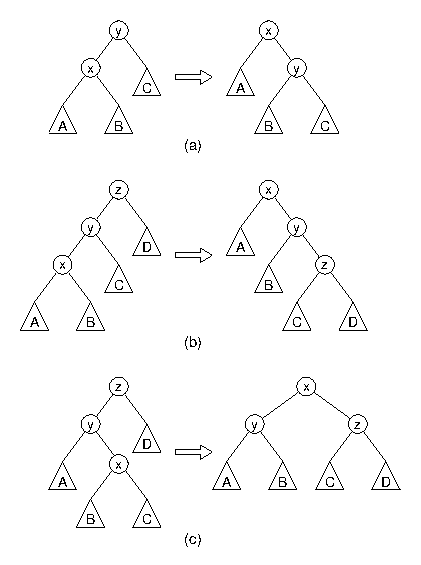
\includegraphics{images/fig1.eps}}
%% \caption{
%% ボトムアップ扁平化操作の1ステップ. % \cite{ST85}
%% $x$ がアクセスした節点.(a) zig: 1回の右回転($y$が根の場合
%% のみ),
%% (b) zig-zig: 枝$yz$と枝$xy$をこの順に右回転,(c) zig-zag: 枝$xy$
%% を左回転し,できた枝$xz$を右回転.}
%% \label{figure:splaying}
%% \end{figure}

%% 扁平化はボトムアップな変形操作であるため,並列操作には適さない.
%% 文献\Cite{ST85}はトップダウン扁平化も提案しているが,これは実装の
%% 容易化が主な目的であり,木の根は操作終了の直前まで確定しない.


%% \subsection{並列操作に関する過去の研究}\label{subsection:related-parallel}

%% 和田\cite{W90}は,並行論理型言語\cite{S89}の論理変数を用いた扁
%% 平化アルゴリズムを提案している.これは,論理変数を利用して,
%% トップダウン扁平化をin-placeで行なうようにしたものと見なすこともできる
%% が,${\it update\/}$のように,対象となる節点が操作終了後の木に存在するこ
%% とがわかっている場合は,木の根のキーを操作の最初に確定させる点が大きな特徴で
%% ある.
%% %
%% % 数百節点の連続挿入操作の並列度は4〜8であるという実験結果が
%% % 報告されている\cite{W90}.
%% %
%% しかしこの技法は,
%% ${\it delete\/}$のように,操作結果の木の根が事前にわから
%% ない場合には適用できない.


%% \subsection{トップダウン扁平化の問題点}

%% トップダウン扁平化による${\it update\/}$は,
%% \ref{subsection:related-parallel}節のように
%% 根のキーを最初に確定させるよ
%% うにしても,並列処理の観点からは問題が残る.たとえば,節点
%% $x(<b)$ ($<$はキーによる順序関係)の${\it update\/}$によって起きる
%% 図\ref{figure:topdown}の
%% zig-zig操作\cite{W90} を考える($L$と$R$は,木$C$をトップダウン扁平
%% 化した結果の左(右)部分木で,${\it update\/}$完了時までに確定).

%% % \begin{adjustvboxheight}
%% \begin{figure}[tb]
%%   \centerline {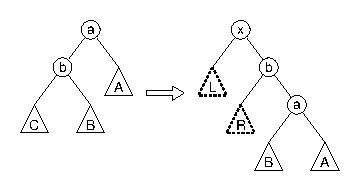
\includegraphics {images/fig2.eps}}
%% \caption{トップダウン扁平化による${\it update\/}$}
%% \label{figure:topdown}
%% \end{figure}
%% % \end{adjustvboxheight}

%% この${\it update\/}$の後,$y(<x)$, $z(>b)$へのアクセスがこの順に続くと
%% する.最初の$x$へのアクセス時に$x$が部分木$C$の左の方にあったためにzig-zig操作
%% が続く場合,$L$の
%% 根が確
%% 定するのは遅くなる.しかし$L$の根が確定するまでは,次の$y$へのアクセ
%% スがzig, zig-zig, zig-zagのどれをまず適用するか決められない.
%% %
%% % 長く待っても,目標の節点の上昇段数が多ければ問題はないのであるが,
%% % それが
%% %
%% そこで3番目の
%% $z$へのアクセスが,2番目の操作によって影響を受けることのない$b$の右部分
%% 木に向かうにもかかわらず,長時間ブロックしてしまう.

%% 削除操作はさらに問題である.一般に,二分木から節点$x$を削除するには,
%% $x$の左部
%% 分木の最大の節点$y$を探してそれを$x$の場所に移すことが基本とな
%% る.しかし,扁平化の有無にかかわらず,$y$が見つかるまでは$x$の場所
%% にくる新たなキーは確定せず,後続の操作をブロックしてしまう.以下のよう
%% な解決法も考えられるが,いずれもうまく動作しない.

%% \begin{enumerate}
%% \item % {\bf 一時的なキー}
%% $y$が見つかるまで,$x$を一時的なキーとして利用すると,
%% $y\le z\le x$であるような節点$z$への操作を誤った方向へ導く.

%% \item % {\bf 双方向リスト}
%% 各節点が直前と直後のキーをもつ節点へのポインタを保持することによって,
%% $x$の直前の要素$y$に${\rm O}(1)$時間でアクセスできるようにする
%% ことが考えられる.これらのポインタは木
%% の扁平化時に変更する必要がないという特徴がある.
%% %
%% しかしこの方法は逐次操作のときしかうまく動作しない.
%% %
%% % あるプロセスが節点
%% % $x$を削除しようとしたとする.そのプロセスは節点$y$に${\rm O}(1)$時間でア
%% % クセスできるものの,単にそれを削除して$x$のかわりに用いることはできない.
%% % (invisible pointer?)
%% %
%% なぜならこの削除操作の前の操作が$x$と$y$を結
%% ぶパスを下降中で,いずれ$y$に到達するかもしれないからである.
%% \end{enumerate}

%% したがって本論文では,高々${\rm O}(1)$個の節を施錠しつつ,厳密にトップダウ
%% ンに木を変形してゆくアルゴリズムを考えることとする.
